\begin{tikzpicture}[scale=1.2]
  % base: regular pentagon in perspective (y squashed)
  \foreach \i in {0,...,4} {
    \coordinate (B\i) at ({1.2*cos(90+72*\i)},{0.4*sin(90+72*\i)});
  }
  \coordinate (A) at (0,2);
  \draw[thick, blue] (B1) -- (B2) -- (B3) -- (B4);
  \draw[thick, blue, dashed] (B4) -- (B0) -- (B1);
  \foreach \i in {1,2,3,4} { \draw[thick, blue] (A) -- (B\i); }
  \draw[thick, blue, dashed] (A) -- (B0);
  % axis
  \draw[dotted, thick] (0,-1.2) -- (0,2.7);
  \draw[->, red] (0.3,2.35) arc[start angle=-20, end angle=200, x radius=0.32, y radius=0.1];
  \node[red, font=\small] at (0.95,2.45) {$\tfrac{2\pi}{n}$};
\end{tikzpicture}
